\documentclass[aspectratio=169]{beamer}

\usetheme{Madrid}
\usecolortheme{default}
\setbeamertemplate{navigation symbols}{}
\setbeamertemplate{caption}[numbered]

\usepackage{amsmath,amssymb,bm}
\usepackage{booktabs}
\usepackage{graphicx}
\usepackage{tikz}
\usetikzlibrary{arrows.meta,positioning}
\usepackage{caption}
\usepackage{subcaption}

\hypersetup{
    colorlinks=true,
    linkcolor=blue,
    urlcolor=cyan
}
\usepackage{cleveref}

\AtBeginSection[]
{
    \begin{frame}{Contents}
        \tableofcontents[currentsection]
    \end{frame}
}

\title[Milestone 2]{Bitcoin Transaction Classification with Network Dependence}
\subtitle{Milestone 2}
\author[T. Bai \and S. Bhowal \and N. Nguyen]{Tian Bai \and Sanchayan Bhowal \and Nathan Nguyen}
\date{}

\begin{document}

\begin{frame}
  \titlepage
\end{frame}

\begin{frame}{Contents}
    \tableofcontents
\end{frame}

\section{Data Description}
\begin{frame}{Data description}
\begin{itemize}
    \item The data comes from the \href{https://pytorch-geometric.readthedocs.io/en/stable/generated/torch_geometric.datasets.EllipticBitcoinDataset.html}{Elliptic Bitcoin dataset}.
    \item Nodes represent Bitcoin transactions; directed edges represent the flow of Bitcoin from one transaction to another.
    \item A transaction is called \alert{licit} or \alert{illicit} according to the entity initiating the transaction.
    \item The graph has over \textbf{200K nodes}, \textbf{234K edges}, and \textbf{166 anonymous node features}.
    \item Labels are only partially observed:
    \[
        \sigma_i = \begin{cases}
            1, & \text{licit},\\
            -1, & \text{illicit},
        \end{cases}
    \]
\end{itemize}
\end{frame}



% in the frame
\begin{frame}{Transaction Graph}
\begin{figure}
    \centering
    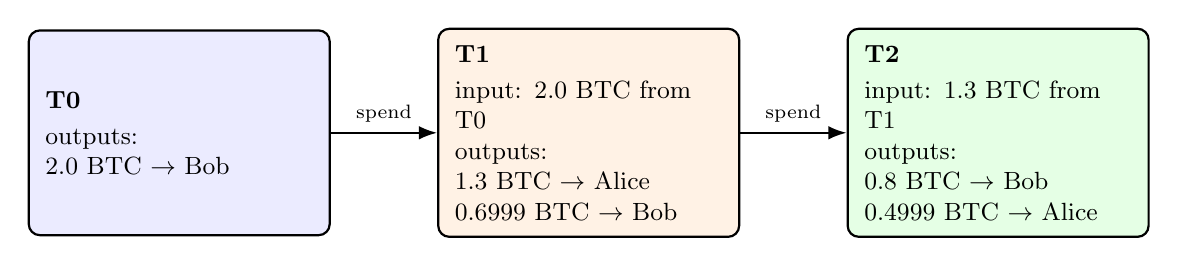
\begin{tikzpicture}[
    >=Latex,
    every node/.style={font=\small},
    txn/.style={
        draw,
        rounded corners,
        thick,
        align=left,
        text width=3.4cm,
        inner sep=6pt,
        minimum height=2.6cm
    }
]

\node[txn, fill=blue!8] (T0) at (0,0) {%
\textbf{T0}\\[2pt]
outputs:\\
$2.0$ BTC $\to$ Bob
};

\node[txn, fill=orange!10] (T1) at (5.2,0) {%
\textbf{T1}\\[2pt]
input: $2.0$ BTC from T0\\
outputs:\\
$1.3$ BTC $\to$ Alice\\
$0.6999$ BTC $\to$ Bob
};

\node[txn, fill=green!10] (T2) at (10.4,0) {%
\textbf{T2}\\[2pt]
input: $1.3$ BTC from T1\\
outputs:\\
$0.8$ BTC $\to$ Bob\\
$0.4999$ BTC $\to$ Alice
};

\draw[->, thick] (T0.east) -- node[above] {\scriptsize spend} (T1.west);
\draw[->, thick] (T1.east) -- node[above] {\scriptsize spend} (T2.west);

\end{tikzpicture}
\caption{A schematic of transaction graph}
\end{figure}
\begin{figure}
    \resizebox{0.4\textwidth}{!}{%
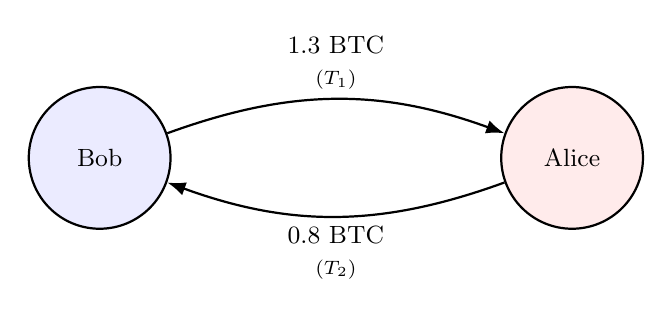
\begin{tikzpicture}[
    >=Latex,
    every node/.style={font=\small},
    ent/.style={
        draw,
        circle,
        thick,
        minimum size=1.8cm,
        align=center
    }
]

\node[ent, fill=blue!8]  (Bob)   at (0,0) {Bob};
\node[ent, fill=red!8]   (Alice) at (6,0) {Alice};

\draw[->, thick] (Bob) to[bend left=20]
    node[above, align=center] {$1.3$ BTC\\ \scriptsize $(T_1)$} (Alice);

\draw[->, thick] (Alice) to[bend left=20]
    node[below, align=center] {$0.8$ BTC\\ \scriptsize $(T_2)$} (Bob);

\end{tikzpicture}%
}
\caption{Money flow between accounts}
\end{figure}
\end{frame}

\section{Exploratory Data Analysis}
\begin{frame}{Network Components}
\begin{figure}
    \centering
    \begin{subfigure}[b]{0.48\textwidth}
        \centering
        
\includegraphics[width=\textwidth]{figures/elliptic_components/component_03.png}
        \phantomcaption
        \label{fig:net_comp1}
    \end{subfigure}
    \hfill
    \begin{subfigure}[b]{0.48\textwidth}
        \centering
        
\includegraphics[width=\textwidth]{figures/elliptic_components/component_02.png}
        \phantomcaption
        \label{fig:net_comp2}
    \end{subfigure}
    \caption{Visualization of network components and the labels.}
\end{figure}
\end{frame}


\begin{frame}{Feature Correlation}
    \begin{figure}
         \centering
    
\includegraphics[width=0.54\textwidth]{figures/feature_correlation.png}
         \phantomcaption
         \label{fig:heatmap}
     \end{figure}
\end{frame}

\begin{frame}{Feature Visualization}
    \begin{figure}
         \centering
    
\includegraphics[width=0.95\textwidth]{figures/PCA.png}
         \phantomcaption
         \label{fig:pca}
     \end{figure}
\end{frame}


\begin{frame}{Glimpse of Neighborhood}
\small
\begin{table}[htbp]
\centering
\caption{Example node-level neighborhood features}
\begin{tabular}{rrrrrr}
\toprule
idx & node & node label & labeled neighbors & illicit neighbors & \% illicit neighbor \\
\midrule
0 & 3  & licit & 62 & 1 & 0.0161 \\
1 & 9  & licit & 23 & 0 & 0.0 \\
2 & 10 & licit & 2  & 0 & 0.0 \\
263 & 907   & illicit & 1 & 0 & 0.0  \\
391 & 1361  & illicit & 1 & 0 & 0.0  \\
\bottomrule
\end{tabular}
\label{table:node}
\end{table}
\end{frame}

\begin{frame}{Evidence of Homophily}

    \begin{table}[htbp]
\centering
\caption{Neighborhood summary by node label}
\resizebox{\textwidth}{!}{%
\begin{tabular}{lrrrrr}
\toprule
node label & nodes & labeled neighbor & illicit neighbor & \% neighbor illicit & \% has illicit neighbor \\
\midrule
illicit & 4545  & 0.8123 & 0.4392 & 0.5097 & 0.3001  \\
licit   & 42019 & 1.6553 & 0.0404 & 0.0181 & 0.0244  \\
\bottomrule
\end{tabular}%
}
\label{table:neighbor}
\end{table}
\end{frame}
\begin{frame}{Evidence of Homophily}
\small
\begin{table}[htbp]
\centering
\caption{Transition counts between labeled source and target nodes}
\begin{tabular}{lrr}
\toprule
source/target & licit & illicit \\
\midrule
licit   & 33930 & 1228 \\
illicit & 468   & 998 \\
\bottomrule
\end{tabular}
\label{table:transition}
\end{table}
\end{frame}

\section{Model Description}
\begin{frame}{Model Sketch}
\small
Assume $\sigma_i \in \{-1,1\}$ is the label of transaction $i$, where $-1$ denotes the illicit class and $1$ denotes the licit class.

\vspace{0.15cm}
We model the joint law of the labels given the features $X$ and graph $G$ by
\[
    P(\sigma_1,\sigma_2,\ldots,\sigma_n \mid X,G)
    \propto \prod_{(i,j)\in E} \psi_{X_i,X_j}(\sigma_i,\sigma_j).
\]

For binary labels, write the pairwise potential as
\[
    \psi_{X_i,X_j}(\sigma_i,\sigma_j)
    = \exp\!\left(\beta_{ij}\sigma_i\sigma_j + \alpha^{(1)}_{ij}\sigma_i+\alpha^{(2)}_{ij}\sigma_j + c_{ij}\right).
\]

Assuming a common network parameter $\beta_{ij}=\beta$ for all $(i,j)\in E$, we obtain
\[
P(\sigma \mid X,G)
\propto
\exp\!\left(
\beta \sum_{(i,j)\in E} \sigma_i\sigma_j
+ 2\sum_{i=1}^n \sigma_i \sum_{j:(i,j)\in E} (\alpha^{(1)}_{ij}+\alpha^{(2)}_{ji})
\right).
\]
\end{frame}

\begin{frame}{Model Sketch}
\small
Model the node-level effect by
\[
     \sum_{j:(i,j)\in E} (\alpha^{(1)}_{ij}+\alpha^{(2)}_{ji}) = X_i^T\gamma,
\]
where $\gamma$ captures the effect of the anonymous features on the labels.

\vspace{0.2cm}
Substituting this into the previous expression gives
\[
    P(\sigma_1,\sigma_2,\ldots,\sigma_n \mid X,G)
    \propto
    \exp\!\left(
        \beta \sum_{(i,j)\in E} \sigma_i\sigma_j
        + \sum_{i=1}^n \sigma_i X_i^T\gamma
    \right).
\]

\begin{itemize}
    \item The first term encodes \alert{network dependence}.
    \item The second term encodes the contribution of \alert{covariates}.
    \item Some of the $\sigma_i$'s are unknown.
\end{itemize}
\end{frame}

\begin{frame}{Conclusion}
\begin{itemize}
    \item The Bitcoin transaction graph is large, sparse, and only partially labeled.
    \item \Cref{fig:net_comp1,fig:net_comp2} suggest that the graph is acyclic.
    \item \Cref{fig:heatmap} shows that the covariates have less correlation.
    \item \Cref{table:neighbor,table:transition} provide strong empirical evidence of homophily.
    \item This motivates a model that combines:
    \begin{itemize}
        \item a covariate term through $\gamma$, and
        \item a network interaction term through $\beta$.
    \end{itemize}
    \item Next step: estimate the parameters and compare with other methods.
\end{itemize}
\end{frame}

\end{document}
